\par{The internal \emph{kernel} is the dominant \emph{kernel} in this implementation of the 
    LU decomposition. It accounts for the majority of computation time. 
    It operates on a larger amount of data than each of the other \emph{kernels}
    and is also very inefficient, in spite of a higher level of parallelism 
    compared to other \emph{kernels}.}

\begin{figure}[!h]
    \centering
    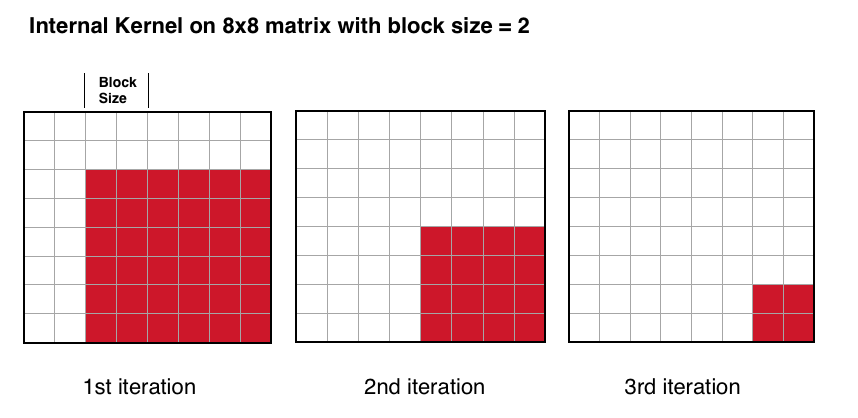
\includegraphics[width=0.6\textwidth]{figures/InternalKernel2.png}
    \caption{Internal \emph{kernel} algorithm on 8x8 matrix with block size = 2.}
    \label{InternalKernel2}
\end{figure}

\par{The first instance of the internal \emph{kernel} operates on the 1st portion of 
    the matrix shown in figure \ref{InternalKernel2}. All \emph{kernels} are enqueued multiple 
    times, so, the next iteration will operate on a portion of the 
    matrix that has been decreased by block size in each dimension.}

\par{Table \ref{tab:lu3} summarises the relevant parameters.}

\begin{table}[!h]
    \centering
    \begin{tabular}{| c | c | c | c |}
    \hline
    \emph{Block Size} & \emph{Data Block / Work Group} & 
    \emph{Starting Number of Work Groups} & 
    \emph{\#Work-Items / Work-Group} \\ \hline
    2 & 3x(2x2) & 4,190,209 & 4 \\ \hline
    4 & 3x(4x4) & 1,046,529 & 16 \\ \hline
    8 & 3x(8x8) & 261,121 & 64 \\ \hline
    16 & 3x(16x16) & 65,025 & 256 \\ \hline
    32 & 3x(32x32) & 16,129 & 1024 \\ \hline
    64 & 3x(64x64) & 3,969 & 4096 \\ \hline
    \end{tabular}
    \caption{Internal \emph{kernal} summary.}
    \label{tab:lu3}
\end{table}

\par{The first thing to note is that the number of \emph{work groups} is very high, 
    which means that the algorithm can exploit the available parallelism 
    in the Xeon CPU and Xeon Phi relatively well. There are almost always 
    enough \emph{work groups} to fill the available hardware threads. As a result, 
    the number of GFLOPS is significantly higher in executions of the internal 
    \emph{kernel} than in executions of the other \emph{kernels}, which do not exploit the 
    parallelism to the same extent. This is a clear demonstration of the 
    performance gains possible from correct utilisation of 
    the available hardware. Table \ref{tab:lu4} compares the number of 
    GFLOPS between executions of the diagonal \emph{kernel} and the internal 
    \emph{kernel} on the Xeon CPU.}

\begin{table}[!h]
    \centering
    \begin{tabular}{| c | c | c | c |}
    \hline
    \emph{Block Size} & \emph{Diagonal} & \emph{Internal} \\ \hline
    2 & 0.00005 & 8.40286 \\ \hline
    4 & 0.00057 & 16.53493 \\ \hline
    8 & 0.00172 & 26.83808 \\ \hline
    16 & 0.03334 & 29.94455 \\ \hline
    32 & 0.11905 & 28.50387 \\ \hline
    64 & 0.30937 & 26.86795 \\ \hline
    \end{tabular}
    \caption{Comparison of GFLOPS, diagonal vs internal \emph{kernels}.}
    \label{tab:lu4}
\end{table}

\par{Clearly, the internal \emph{kernel} is achieving higher performance 
    figures than the previously discussed diagonal \emph{kernel}, which 
    only uses 1 out of 40 hardware threads on the Xeon CPU.}

\par{In spite of this, the internal \emph{kernel} is clearly not an optimal 
    algorithm. When the \emph{work groups} are first enqueued, the \emph{kernels} 
    operate on a very large block of data. In the next iteration of 
    the loop, the \emph{kernels} operate on almost the same block of data, 
    albeit decreased by block size in each dimension. Thus, 
    the \emph{kernel} is operating multiple times on almost the same blocks of data.}

\par{The total number of floating point operations that the internal \emph{kernel} 
    performs reduces with the block size, since the number of redundant 
    operations reduces.}

\par{Figure \ref{InternalKernel1} below shows the total computation 
    times for the internal \emph{kernel} on each of the three devices.}

\begin{figure}[!h]
    \centering
    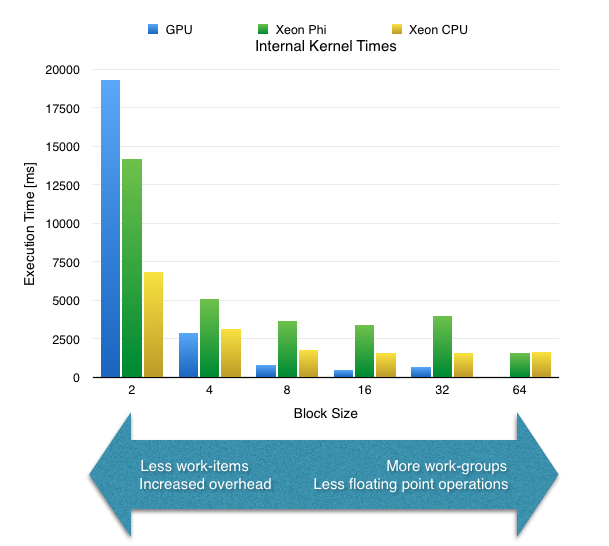
\includegraphics[width=0.6\textwidth]{figures/InternalKernel1.png}
    \caption{4096x4096 Internal \emph{kernel} times.}
    \label{InternalKernel1}
\end{figure}

\par{The above graph highlights some interesting points. It is clear to 
    see that when the number of \emph{work items} is minimised (block size 2), 
    the GPU offers the worst performance. As mentioned previously, optimal 
    performance on the GPU is achieved with a large number of \emph{work items} 
    per \emph{work group}. Significant performance improvements are seen on the GPU 
    as the number of \emph{work items} per \emph{work group} increases.}

\par{Another interesting point to note is that, as the block size 
    increases, the performance of the Xeon CPU and Xeon Phi improves. 
    This is not only due to the decrease in floating point operations, 
    but also due to the increase in \emph{work items} per \emph{work group} whilst still 
    maintaining a large number of \emph{work groups}. Intel’s SDK for OpenCL 
    applications states that:}

\par{\emph{``To reduce the overhead of maintaining a \emph{work group}, create 
    \emph{work groups} that are as large as possible. Still there should be 
    a sufficient number of \emph{work groups}."}}

\par{The internal \emph{kernel} satisfies these conditions for large block sizes 
    and the performance improves as a result.}

